\documentclass[border=5pt]{standalone}
\usepackage[T1]{fontenc}
\usepackage{lmodern,amsmath}
\usepackage{pgfplots}
\pgfplotsset{compat=1.18}
\usepgfplotslibrary{fillbetween}
\begin{document}
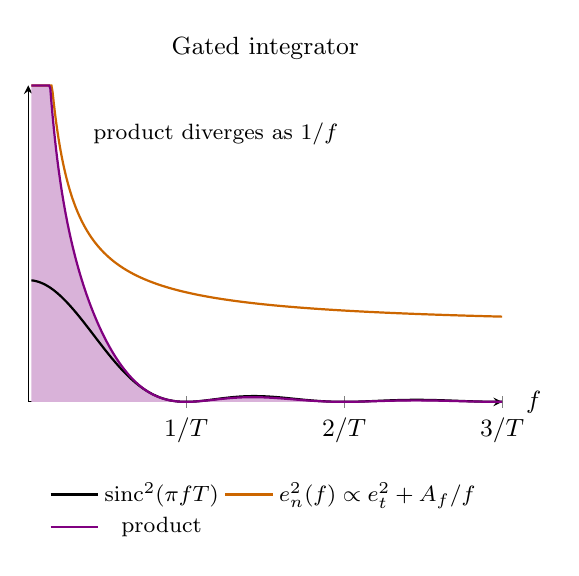
\begin{tikzpicture}[font=\small]
\begin{axis}[width=7.6cm,height=5.6cm,
  xmin=0,xmax=3,ymin=0,ymax=2.6,
  xtick={1,2,3},xticklabels={$1/T$,$2/T$,$3/T$},ytick=\empty,
  xlabel={$f$},xlabel style={at={(axis description cs:1.03,0)},anchor=west},axis lines=left,clip=false,
  title={Gated integrator},
  legend style={at={(0.5,-0.22)},anchor=north,draw=none,fill=none,font=\footnotesize,legend columns=2},
  samples=400,domain=0.02:3]
\addplot[black,thick] {(sin(deg(pi*x))/(pi*x))^2};
\addlegendentry{$\mathrm{sinc}^2(\pi fT)$}
\addplot[orange!80!black,thick] {min(2.6,0.6*(1+0.5/x))};
\addlegendentry{$e_n^2(f)\propto e_t^2+A_f/f$}
\addplot[name path=P,violet,thick] {min(2.6,0.6*(1+0.5/x)*(sin(deg(pi*x))/(pi*x))^2)};
\addlegendentry{product}
\path[name path=Z] (axis cs:0.02,0) -- (axis cs:3,0);
\addplot[violet!30] fill between[of=P and Z];
\node[anchor=west,font=\footnotesize,align=left] at (axis cs:0.35,2.2) {product diverges as $1/f$};
\end{axis}
\end{tikzpicture}\hspace{8mm}%
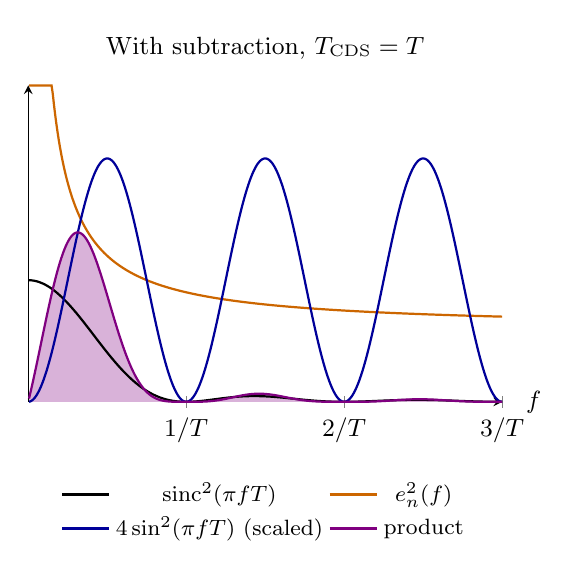
\begin{tikzpicture}[font=\small]
\begin{axis}[width=7.6cm,height=5.6cm,
  xmin=0,xmax=3,ymin=0,ymax=2.6,
  xtick={1,2,3},xticklabels={$1/T$,$2/T$,$3/T$},ytick=\empty,
  xlabel={$f$},xlabel style={at={(axis description cs:1.03,0)},anchor=west},axis lines=left,clip=false,
  title={With subtraction, $T_{\rm CDS}=T$},
  legend style={at={(0.5,-0.22)},anchor=north,draw=none,fill=none,font=\footnotesize,legend columns=2},
  samples=400,domain=0.005:3]
\addplot[black,thick] {(sin(deg(pi*x))/(pi*x))^2};
\addlegendentry{$\mathrm{sinc}^2(\pi fT)$}
\addplot[orange!80!black,thick] {min(2.6,0.6*(1+0.5/x))};
\addlegendentry{$e_n^2(f)$}
\addplot[blue!60!black,thick] {min(2.6,0.5*4*(sin(deg(pi*x)))^2)};
\addlegendentry{$4\sin^2(\pi fT)$ (scaled)}
\addplot[name path=Q,violet,thick] {0.45*0.6*(1+0.5/x)*(sin(deg(pi*x))/(pi*x))^2*4*(sin(deg(pi*x)))^2};
\addlegendentry{product}
\path[name path=Z2] (axis cs:0.005,0) -- (axis cs:3,0);
\addplot[violet!30] fill between[of=Q and Z2];
\end{axis}
\end{tikzpicture}
\end{document}
